% Options for packages loaded elsewhere
\PassOptionsToPackage{unicode}{hyperref}
\PassOptionsToPackage{hyphens}{url}
%
\documentclass[
]{article}
\usepackage{amsmath,amssymb}
\usepackage{lmodern}
\usepackage{iftex}
\ifPDFTeX
  \usepackage[T1]{fontenc}
  \usepackage[utf8]{inputenc}
  \usepackage{textcomp} % provide euro and other symbols
\else % if luatex or xetex
  \usepackage{unicode-math}
  \defaultfontfeatures{Scale=MatchLowercase}
  \defaultfontfeatures[\rmfamily]{Ligatures=TeX,Scale=1}
\fi
% Use upquote if available, for straight quotes in verbatim environments
\IfFileExists{upquote.sty}{\usepackage{upquote}}{}
\IfFileExists{microtype.sty}{% use microtype if available
  \usepackage[]{microtype}
  \UseMicrotypeSet[protrusion]{basicmath} % disable protrusion for tt fonts
}{}
\makeatletter
\@ifundefined{KOMAClassName}{% if non-KOMA class
  \IfFileExists{parskip.sty}{%
    \usepackage{parskip}
  }{% else
    \setlength{\parindent}{0pt}
    \setlength{\parskip}{6pt plus 2pt minus 1pt}}
}{% if KOMA class
  \KOMAoptions{parskip=half}}
\makeatother
\usepackage{xcolor}
\usepackage[margin=1in]{geometry}
\usepackage{color}
\usepackage{fancyvrb}
\newcommand{\VerbBar}{|}
\newcommand{\VERB}{\Verb[commandchars=\\\{\}]}
\DefineVerbatimEnvironment{Highlighting}{Verbatim}{commandchars=\\\{\}}
% Add ',fontsize=\small' for more characters per line
\usepackage{framed}
\definecolor{shadecolor}{RGB}{248,248,248}
\newenvironment{Shaded}{\begin{snugshade}}{\end{snugshade}}
\newcommand{\AlertTok}[1]{\textcolor[rgb]{0.94,0.16,0.16}{#1}}
\newcommand{\AnnotationTok}[1]{\textcolor[rgb]{0.56,0.35,0.01}{\textbf{\textit{#1}}}}
\newcommand{\AttributeTok}[1]{\textcolor[rgb]{0.77,0.63,0.00}{#1}}
\newcommand{\BaseNTok}[1]{\textcolor[rgb]{0.00,0.00,0.81}{#1}}
\newcommand{\BuiltInTok}[1]{#1}
\newcommand{\CharTok}[1]{\textcolor[rgb]{0.31,0.60,0.02}{#1}}
\newcommand{\CommentTok}[1]{\textcolor[rgb]{0.56,0.35,0.01}{\textit{#1}}}
\newcommand{\CommentVarTok}[1]{\textcolor[rgb]{0.56,0.35,0.01}{\textbf{\textit{#1}}}}
\newcommand{\ConstantTok}[1]{\textcolor[rgb]{0.00,0.00,0.00}{#1}}
\newcommand{\ControlFlowTok}[1]{\textcolor[rgb]{0.13,0.29,0.53}{\textbf{#1}}}
\newcommand{\DataTypeTok}[1]{\textcolor[rgb]{0.13,0.29,0.53}{#1}}
\newcommand{\DecValTok}[1]{\textcolor[rgb]{0.00,0.00,0.81}{#1}}
\newcommand{\DocumentationTok}[1]{\textcolor[rgb]{0.56,0.35,0.01}{\textbf{\textit{#1}}}}
\newcommand{\ErrorTok}[1]{\textcolor[rgb]{0.64,0.00,0.00}{\textbf{#1}}}
\newcommand{\ExtensionTok}[1]{#1}
\newcommand{\FloatTok}[1]{\textcolor[rgb]{0.00,0.00,0.81}{#1}}
\newcommand{\FunctionTok}[1]{\textcolor[rgb]{0.00,0.00,0.00}{#1}}
\newcommand{\ImportTok}[1]{#1}
\newcommand{\InformationTok}[1]{\textcolor[rgb]{0.56,0.35,0.01}{\textbf{\textit{#1}}}}
\newcommand{\KeywordTok}[1]{\textcolor[rgb]{0.13,0.29,0.53}{\textbf{#1}}}
\newcommand{\NormalTok}[1]{#1}
\newcommand{\OperatorTok}[1]{\textcolor[rgb]{0.81,0.36,0.00}{\textbf{#1}}}
\newcommand{\OtherTok}[1]{\textcolor[rgb]{0.56,0.35,0.01}{#1}}
\newcommand{\PreprocessorTok}[1]{\textcolor[rgb]{0.56,0.35,0.01}{\textit{#1}}}
\newcommand{\RegionMarkerTok}[1]{#1}
\newcommand{\SpecialCharTok}[1]{\textcolor[rgb]{0.00,0.00,0.00}{#1}}
\newcommand{\SpecialStringTok}[1]{\textcolor[rgb]{0.31,0.60,0.02}{#1}}
\newcommand{\StringTok}[1]{\textcolor[rgb]{0.31,0.60,0.02}{#1}}
\newcommand{\VariableTok}[1]{\textcolor[rgb]{0.00,0.00,0.00}{#1}}
\newcommand{\VerbatimStringTok}[1]{\textcolor[rgb]{0.31,0.60,0.02}{#1}}
\newcommand{\WarningTok}[1]{\textcolor[rgb]{0.56,0.35,0.01}{\textbf{\textit{#1}}}}
\usepackage{graphicx}
\makeatletter
\def\maxwidth{\ifdim\Gin@nat@width>\linewidth\linewidth\else\Gin@nat@width\fi}
\def\maxheight{\ifdim\Gin@nat@height>\textheight\textheight\else\Gin@nat@height\fi}
\makeatother
% Scale images if necessary, so that they will not overflow the page
% margins by default, and it is still possible to overwrite the defaults
% using explicit options in \includegraphics[width, height, ...]{}
\setkeys{Gin}{width=\maxwidth,height=\maxheight,keepaspectratio}
% Set default figure placement to htbp
\makeatletter
\def\fps@figure{htbp}
\makeatother
\setlength{\emergencystretch}{3em} % prevent overfull lines
\providecommand{\tightlist}{%
  \setlength{\itemsep}{0pt}\setlength{\parskip}{0pt}}
\setcounter{secnumdepth}{-\maxdimen} % remove section numbering
\ifLuaTeX
  \usepackage{selnolig}  % disable illegal ligatures
\fi
\IfFileExists{bookmark.sty}{\usepackage{bookmark}}{\usepackage{hyperref}}
\IfFileExists{xurl.sty}{\usepackage{xurl}}{} % add URL line breaks if available
\urlstyle{same} % disable monospaced font for URLs
\hypersetup{
  pdftitle={Introduction à R},
  pdfauthor={ibrahima SAGNO},
  hidelinks,
  pdfcreator={LaTeX via pandoc}}

\title{Introduction à R}
\author{ibrahima SAGNO}
\date{2023-06-26}

\begin{document}
\maketitle

{
\setcounter{tocdepth}{2}
\tableofcontents
}
\hypertarget{quest---ce-que-r}{%
\subsection{Qu'est - ce que R ?}\label{quest---ce-que-r}}

Développé par \textbf{Ross Lhaka} et \textbf{Robert Gentleman} à
l'université d'Auckland, en Nouvelle-Zélande dans les années 1990, R est
d'abord un langage de programmation et un environnement logiciel ``Open
source''. Il a été conçu pour l'\textbf{analyse statistique , la
manipulation des données et la visualisation}. L'appelation
\textbf{``Open source''} désigne un logiciel ou un programme dont la
conception,le code source et les droits de distribution sont ouverts et
accessibles à tous.

A cet effet, R dispose d'une grande communauté d'utilisateurs. EN
naviguant sur le web , vous trouverez des forums, des listes de
diffusion, ou encore des groupes dédiées à R dans lesquels vous
trouverez réponse à la plupart de vos inquiétudes.

De plus, R est largement utilisé dans le monde universitaire et dans le
monde de la recherche là où on fait beaucoup appel à des préceptes
statistiques.

\hypertarget{pourquoi-r}{%
\subsection{Pourquoi R ?}\label{pourquoi-r}}

Il existe pluisieurs langages de programmation des plus simples au plus
complexe. Pourquoi alors le choix d'écrire un livre sur R ? Il y'a des
années maintenant que j'ai pour ambition d'initier un public non initié
aux concetps de l'Analytics. Cependant, R est le langage qui se
rapproche le plus des fomules \textbf{Excel} que nous utilisons depuis
le collège. C'est pour cette raison pédagogique et linéaire que mon
choix porte sur R d'autant plus que c'est le prmier langage que j'ai
appris durant mes années de licence.

\hypertarget{que-contient-ce-livre}{%
\subsection{Que contient ce livre ?}\label{que-contient-ce-livre}}

Ce livre a l'avantage d'être concis et à la fois. Il comprendra 7
chapitres allant de l'installation de R Studio, aux utilisations
avancées de R à savoir la création des fonctions, l'utlisation des
boucles en passant par l'analyse statistique et la visualisation des
données.

Comme je le disais en Introduction, R est un logiciel open source.
Durant le déroulé de ce livre, nous utiliserons principalement des
``Packages'' , c'est à dire des bibliothèques conçues par la communauté
et regroupant plusieurs fonctionnalités.

\hypertarget{chapitre-1-installation-et-configuration-de-r}{%
\subsection{Chapitre 1: Installation et Configuration de
R}\label{chapitre-1-installation-et-configuration-de-r}}

Vous pouvez installer \textbf{R} sur les principales distributions à
savoir Windows, macOS, et Linux.

\hypertarget{tuxe9luxe9chargement-de-r}{%
\subsubsection{Téléchargement de R:}\label{tuxe9luxe9chargement-de-r}}

Pour télécharger le programme d'installation de R, rendez-vous sur le
site officiel du \href{https://www.r-project.org/}{projet R}.

\begin{itemize}
\tightlist
\item
  Cliquez sur le lien de téléchargement correspondant à votre système
  d'exploitation (Windows, macOS, Linux).\\
\item
  Choisissez un miroir de téléchargement proche de votre emplacement
  géographique en cliquant sur le lien
  \href{https://cran.r-project.org/mirrors.html}{CRAN}. Le lien vers la
  France est disponible \href{https://pbil.univ-lyon1.fr/CRAN/}{ici}.\\
\item
  Téléchargez le fichier d'installation de R correspondant à votre
  système d'exploitation.
\end{itemize}

\hypertarget{installation-de-r}{%
\subsubsection{Installation de R}\label{installation-de-r}}

\begin{itemize}
\tightlist
\item
  Exécuter le fichier d'installation téléchargé\\
\item
  Suivez les instructions de l'assisstant d'installation pour configurer
  R sur votre système d'exploitation.\\
\item
  Choississez votre repertoire d'installation et les options de
  configuration selon vos préférences.
\end{itemize}

\hypertarget{configuration-de-lenvironnement-de-duxe9veloppement-intuxe9gruxe9-ide-studio}{%
\subsubsection{Configuration de l'environnement de développement intégré
(IDE
Studio)}\label{configuration-de-lenvironnement-de-duxe9veloppement-intuxe9gruxe9-ide-studio}}

un IDE fourni un ensemble d'outils , d'éditeurs de code, de débogueurs ,
de consoles et d'autres fonctionnalités pour aider les utilisateurs à
écrire, tester et déployer leur code de manière plus éfficace. Un IDE à
l'avantage d'être ludique et permet l'autocomplétion des commandes
écrites.

R dispose d'un IDE spécifique appelé \textbf{Rstudio}. Vous pouvez
également éxécuter du code R sur divers autres IDE comme Notepad++,
VScode, etc.\\
Pour télécharger l'IDE Rstudio , rendez-vous sur le site officiel de
Rsudio (\url{https://www.rstudio.com/}). Cliquez sur \textbf{Download
RStudio} et choisissez votre système d'exploitation. Puis installez
Rstudio en suivant les instructions d'installation spécifiques à votre
système d'exploitation.

\hypertarget{premiuxe8re-prise-en-main-hello-word}{%
\subsubsection{Première prise en main: Hello
word!!}\label{premiuxe8re-prise-en-main-hello-word}}

Une fois R et Rstudio installés , lancez R ou Rstudio. Tapez une
commande basique du type \emph{print(`Hello Word')} dans la console. Si
ceci s'exécute sans message d'erreur. Alors votre installation est
correcte.

\begin{Shaded}
\begin{Highlighting}[]
\FunctionTok{print}\NormalTok{(}\StringTok{"Hello word"}\NormalTok{)}
\end{Highlighting}
\end{Shaded}

\begin{verbatim}
## [1] "Hello word"
\end{verbatim}

\hypertarget{pruxe9sentation-de-lenvironnement-rstudio}{%
\subsubsection{Présentation de l'environnement
RStudio}\label{pruxe9sentation-de-lenvironnement-rstudio}}

L'interface de Rstudio se présente en 4 blocs à savoir :

\begin{itemize}
\item
  Bloc 1: L'éditeur de texte\\
  Le Bloc 1 permet d'écrire votre code \textbf{R} de façon propre,
  lisible. Elle permet de garder une trace de votre script.
\item
  Bloc 2: La console\\
  La console permet d'éxécuter votre script R. Un message d'erreur
  s'affichera lorsque votre code contient des erreurs.
\item
  Bloc 3: L'environnement\\
  Le bloc 3 permet de stocker vos variables crées lors d'une session R.
  Elle donne également un aperçu de toutes les données importées ou
  crées.
\item
  Bloc 4: Liste des dossiers/Packages/Visualisation des graphes/Aide\\
  Le Bloc 4 permet tout d'abord de naviguer dans les dossiers de votre
  ordinateur à travers l'onglet \textbf{Files}. l'onglet
  \textbf{Packages} de ce bloc donne la liste de tous les packages
  disponibles sur votre version de R.Dès lors, vous pouvez choisir de
  les installer pour une utilisation future.\\
  L'onglet \textbf{Plot} permet une visualisation des graphiques que
  vous affichez. Et enfin \textbf{Help} est l'aide native de R. Elle
  donne une documentation complète de toutes les fonctions disponibles
  sous R.
\end{itemize}

\begin{figure}
\centering
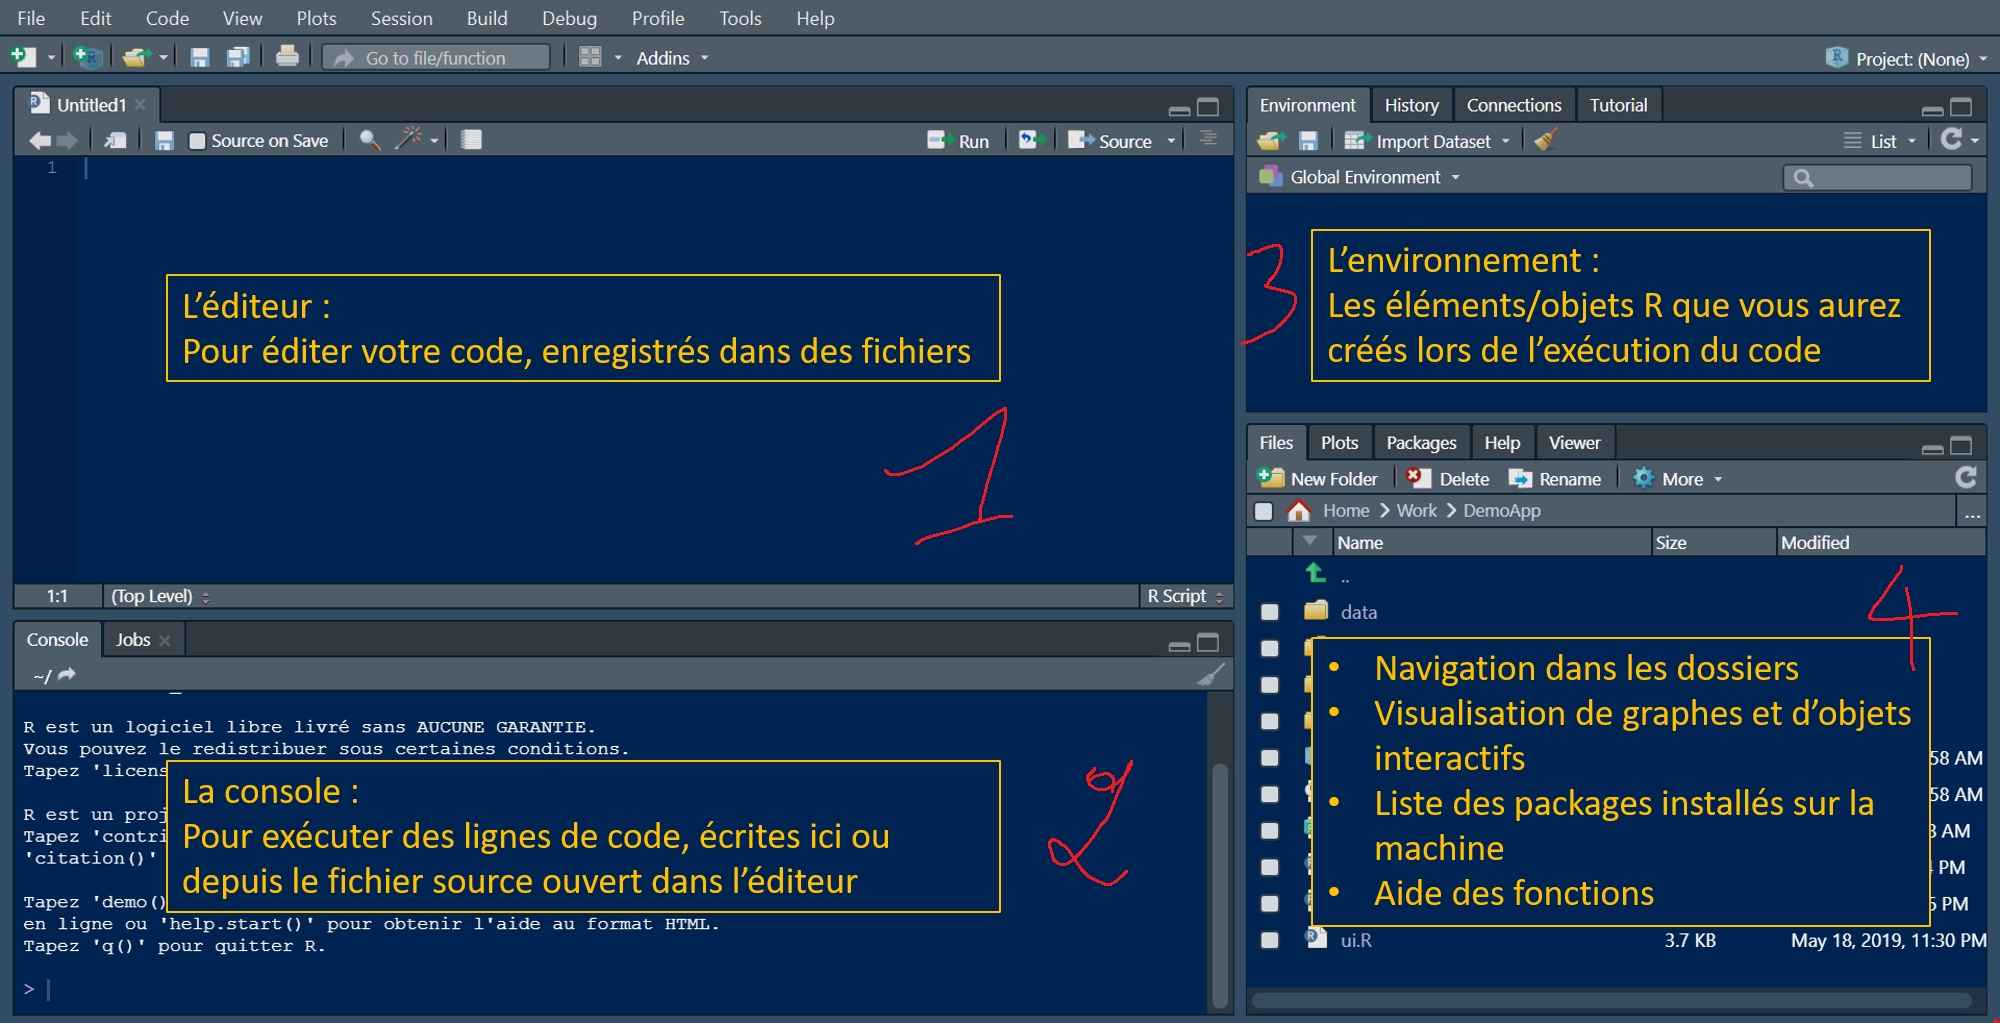
\includegraphics{interface Rstudio.png}
\caption{interface de Rstudio}
\end{figure}

\hypertarget{bases-de-r-et-langage-native}{%
\subsection{Bases de R et langage
native}\label{bases-de-r-et-langage-native}}

Lorsqu'on apprend une nouvelle langue , nous sommes excités à l'idée de
pouvoir employer les. mots appris. Tel est le cas pour tout langage de
programmation. Le logiciel ne comprend que la langue qui lui est dédié.
Donc si vous ne voulez pas voir votre console pleine de ``messages
d'erreur'', vous avez intérêt à écrire dans une langue dans laquelle
elle comprend.

Vous allez donc apprendre à écrire vos premières lignes de code.

\hypertarget{syntaxe-de-base}{%
\subsubsection{Syntaxe de base}\label{syntaxe-de-base}}

Les syntaxes de base de R sont très simples. Nous avons:\\
1. L'assignation de valeurs à une variable\\
Pour assigner une valeur à une variable , on donne un nom à la variable
et on lui ``attribue'' la valeur que l'on souhaite. La règle à retenir
est de ne pas laisser d'espace dans le nom de votre variable. Par
exemple, {``Ma variable''} n'est pas un nom de variable valide mais
{``Ma\_variable''} si.

Par exemple , si on veut assigner la valeur 5 à une variable ``nombre''
, on écrira:

\begin{Shaded}
\begin{Highlighting}[]
\NormalTok{nombre }\OtherTok{\textless{}{-}} \DecValTok{5}
\CommentTok{\#ou }
\NormalTok{nombre }\OtherTok{=} \DecValTok{5}
\end{Highlighting}
\end{Shaded}

\begin{enumerate}
\def\labelenumi{\arabic{enumi}.}
\setcounter{enumi}{1}
\tightlist
\item
  Affichafe des résultats\\
  Pour afficher les résultats ou le contenu d'une variable , il suffit
  de saisir simplement le nom de la variable ou de le précéder de la
  fonction \textbf{print} .
\end{enumerate}

\begin{Shaded}
\begin{Highlighting}[]
\NormalTok{nombre}
\end{Highlighting}
\end{Shaded}

\begin{verbatim}
## [1] 5
\end{verbatim}

\begin{Shaded}
\begin{Highlighting}[]
\CommentTok{\#ou}
\FunctionTok{print}\NormalTok{(nombre)}
\end{Highlighting}
\end{Shaded}

\begin{verbatim}
## [1] 5
\end{verbatim}

\begin{enumerate}
\def\labelenumi{\arabic{enumi}.}
\setcounter{enumi}{2}
\tightlist
\item
  Les commentaires\\
  Lorsqu'on écrit du code , nous mettons des commentaires pour faciliter
  la compréhension de notre script. Ces commentaires ne sont pas
  éxécuter par la console. Pour écrire un texte en commentaire , il
  suffit de le précéder du symbole \textbf{\#}.
\end{enumerate}

\begin{Shaded}
\begin{Highlighting}[]
\CommentTok{\#Ceci est un commentaire}
\end{Highlighting}
\end{Shaded}

\begin{enumerate}
\def\labelenumi{\arabic{enumi}.}
\setcounter{enumi}{3}
\tightlist
\item
  Les opérateurs mathématiques Comme sur une calculatrice, R prend en
  charge toutes les opérations mathématiques à savoir l'addition (+), la
  multiplication (x), la soustraction (-), la division (/) et la
  puissance (\^{}).
\end{enumerate}

\begin{Shaded}
\begin{Highlighting}[]
\CommentTok{\#SUpposons les variables a et b telles que:}
\NormalTok{a }\OtherTok{\textless{}{-}} \DecValTok{20}
\NormalTok{b }\OtherTok{\textless{}{-}} \DecValTok{3}
\CommentTok{\#Alors:}
\NormalTok{c }\OtherTok{\textless{}{-}}\NormalTok{ a }\SpecialCharTok{+}\NormalTok{ b   }\CommentTok{\#Additon}
\NormalTok{d }\OtherTok{\textless{}{-}}\NormalTok{ a }\SpecialCharTok{{-}}\NormalTok{ b   }\CommentTok{\# Soustraction}
\NormalTok{e }\OtherTok{\textless{}{-}}\NormalTok{ a }\SpecialCharTok{*}\NormalTok{ b   }\CommentTok{\# Multiplication}
\NormalTok{f }\OtherTok{\textless{}{-}}\NormalTok{ a }\SpecialCharTok{/}\NormalTok{ b   }\CommentTok{\# Division}
\NormalTok{g }\OtherTok{\textless{}{-}}\NormalTok{ a }\SpecialCharTok{\^{}}\NormalTok{ b   }\CommentTok{\# Puissance}
\NormalTok{i }\OtherTok{\textless{}{-}}\NormalTok{ a }\SpecialCharTok{\%\%}\NormalTok{ b }\CommentTok{\# a modulo b ou le reste de la division de a par b}
\end{Highlighting}
\end{Shaded}

A noter qu'il est possible de réliser les opérations mathématiques les
plus complexes:

\begin{Shaded}
\begin{Highlighting}[]
\CommentTok{\#Supposons la variabe a telle que:}
\NormalTok{a }\OtherTok{\textless{}{-}} \DecValTok{5}
\CommentTok{\#Alors}
\NormalTok{b }\OtherTok{\textless{}{-}} \FunctionTok{log}\NormalTok{(a)   }\CommentTok{\#logarithme néperien (ln) de a }
\NormalTok{c }\OtherTok{\textless{}{-}} \FunctionTok{log10}\NormalTok{(a) }\CommentTok{\#logarithme à base 10 de a }
\NormalTok{d }\OtherTok{\textless{}{-}} \FunctionTok{exp}\NormalTok{(a)   }\CommentTok{\#Exponentielle de a}
\NormalTok{e }\OtherTok{\textless{}{-}} \FunctionTok{sqrt}\NormalTok{(a)  }\CommentTok{\#Racine carrée de a}
\end{Highlighting}
\end{Shaded}

\hypertarget{les-types-de-variables-en-r}{%
\subsection{Les types de variables en
R}\label{les-types-de-variables-en-r}}

Lorsqu'on manipule des données, la première chose à faire est de se
rassurer de leur types. R dispose de plusiers types de données que nous
allons découvrir ensemble.\\
1. Numeric\\
2. Integer\\
3. Character\\
4. Logical

\hypertarget{les-structures-de-donnuxe9es-en-r}{%
\subsection{Les structures de données en
R}\label{les-structures-de-donnuxe9es-en-r}}

\begin{enumerate}
\def\labelenumi{\arabic{enumi}.}
\tightlist
\item
  Les vecteurs\\
\item
  Les matrices\\
\item
  Les listes\\
\item
  Les Factors
\item
  Les Data frames
\end{enumerate}

\hypertarget{manipulation-des-donnuxe9es-avec-r}{%
\subsection{Manipulation des données avec
R}\label{manipulation-des-donnuxe9es-avec-r}}

\hypertarget{importation-des-donnuxe9es-r}{%
\subsubsection{Importation des données
R}\label{importation-des-donnuxe9es-r}}

\hypertarget{exploration-des-donnuxe9es}{%
\subsubsection{Exploration des
données}\label{exploration-des-donnuxe9es}}

\hypertarget{manipulation-des-donnuxe9es}{%
\subsubsection{Manipulation des
données}\label{manipulation-des-donnuxe9es}}

\hypertarget{statistiques-descriptives-avec-r}{%
\subsubsection{Statistiques descriptives avec
R}\label{statistiques-descriptives-avec-r}}

\hypertarget{netoyage-des-donnuxe9es}{%
\subsubsection{Netoyage des données}\label{netoyage-des-donnuxe9es}}

\hypertarget{visualisation-des-donnuxe9es-avec-r}{%
\subsection{Visualisation des données avec
R}\label{visualisation-des-donnuxe9es-avec-r}}

\hypertarget{introduction-aux-graphiques-de-base}{%
\subsubsection{Introduction aux graphiques de
base}\label{introduction-aux-graphiques-de-base}}

\hypertarget{graphiques-avancuxe9s-avec-ggplot2}{%
\subsubsection{Graphiques avancés avec
ggplot2}\label{graphiques-avancuxe9s-avec-ggplot2}}

\hypertarget{programmation-avancuxe9es-avec-r}{%
\subsection{Programmation avancées avec
R}\label{programmation-avancuxe9es-avec-r}}

\hypertarget{les-boucles}{%
\subsubsection{Les boucles}\label{les-boucles}}

\hypertarget{les-fonctions}{%
\subsubsection{Les fonctions}\label{les-fonctions}}

\end{document}
